%===============================================================================
% $Id: ifacconf.tex 19 2011-10-27 09:32:13Z jpuente $  
% Template for IFAC meeting papers
% Copyright (c) 2007-2008 International Federation of Automatic Control
%===============================================================================
\documentclass{ifacconf}

\usepackage{graphicx}      % include this line if your document contains figures
\usepackage{natbib}        % required for bibliography
%===============================================================================
\begin{document}
\begin{frontmatter}

\title{Grupo 3 - Módulo 1 - Massa Mola} 
% Title, preferably not more than 10 words.

%\thanks[footnoteinfo]{Sponsor and financial support acknowledgment
%goes here. Paper titles should be written in uppercase and lowercase
%letters, not all uppercase.}

\author[First]{Felipe Nery Barcelos Araújo (2020021190)} 
\author[First]{Gustavo Vieira Barbosa (2020021352)} 
\author[First]{Matheus Marques Gonçalves de Paula (2020068995)}

\address[First]{
  Engenharia de Controle e Automação,\\ Universidade Federal de Minas Gerais, MG \\
   (e-mails: felipenery@ufmg.br, gustavovbarbosa@ufmg.br, mmgp@ufmg.br)
}

%Escrever um resumo do documento aqui, não pode ultrapassar 250 palavras
\begin{abstract}               
These instructions give you guidelines for preparing papers for IFAC
technical meetings. Please use this document as a template to prepare
your manuscript. For submission guidelines, follow instructions on
paper submission system as well as the event website.
\end{abstract}

%Escrever até 5 palavras chave do relatório aqui
\begin{keyword}
massa-mola, controle, posição
\end{keyword}

\end{frontmatter}

%===============================================================================

\section{Introdução}

Os sistemas massa-mola são capazes de representar uma ampla gama de fenômenos
físicos e engenharia. De forma a desempenhar um papel fundamental na modelagem 
desses fenômenos e sistemas mecânicos complexos, tais como: suspensões veiculares, 
sistemas de suspensão de edifícios, sistemas biomecânicos e muitos outros o sistema 
massa-mola representa com elevada exatidão. Afinal, com uma modelagem precisa, o sistema
é capaz de realizar controle garantindo o desempenho e a estabilidade desejada.

Ao longo desse relatório será visto um estudo focado no controle de um sistema de massa-mola 
composto por duas massas interconectadas por duas molas, como mostra a figura \ref{fig:planta_padrao}, um problema
clássico de controle de sistemas dinâmicos. 

\begin{figure}[!htb]
  \begin{center}
  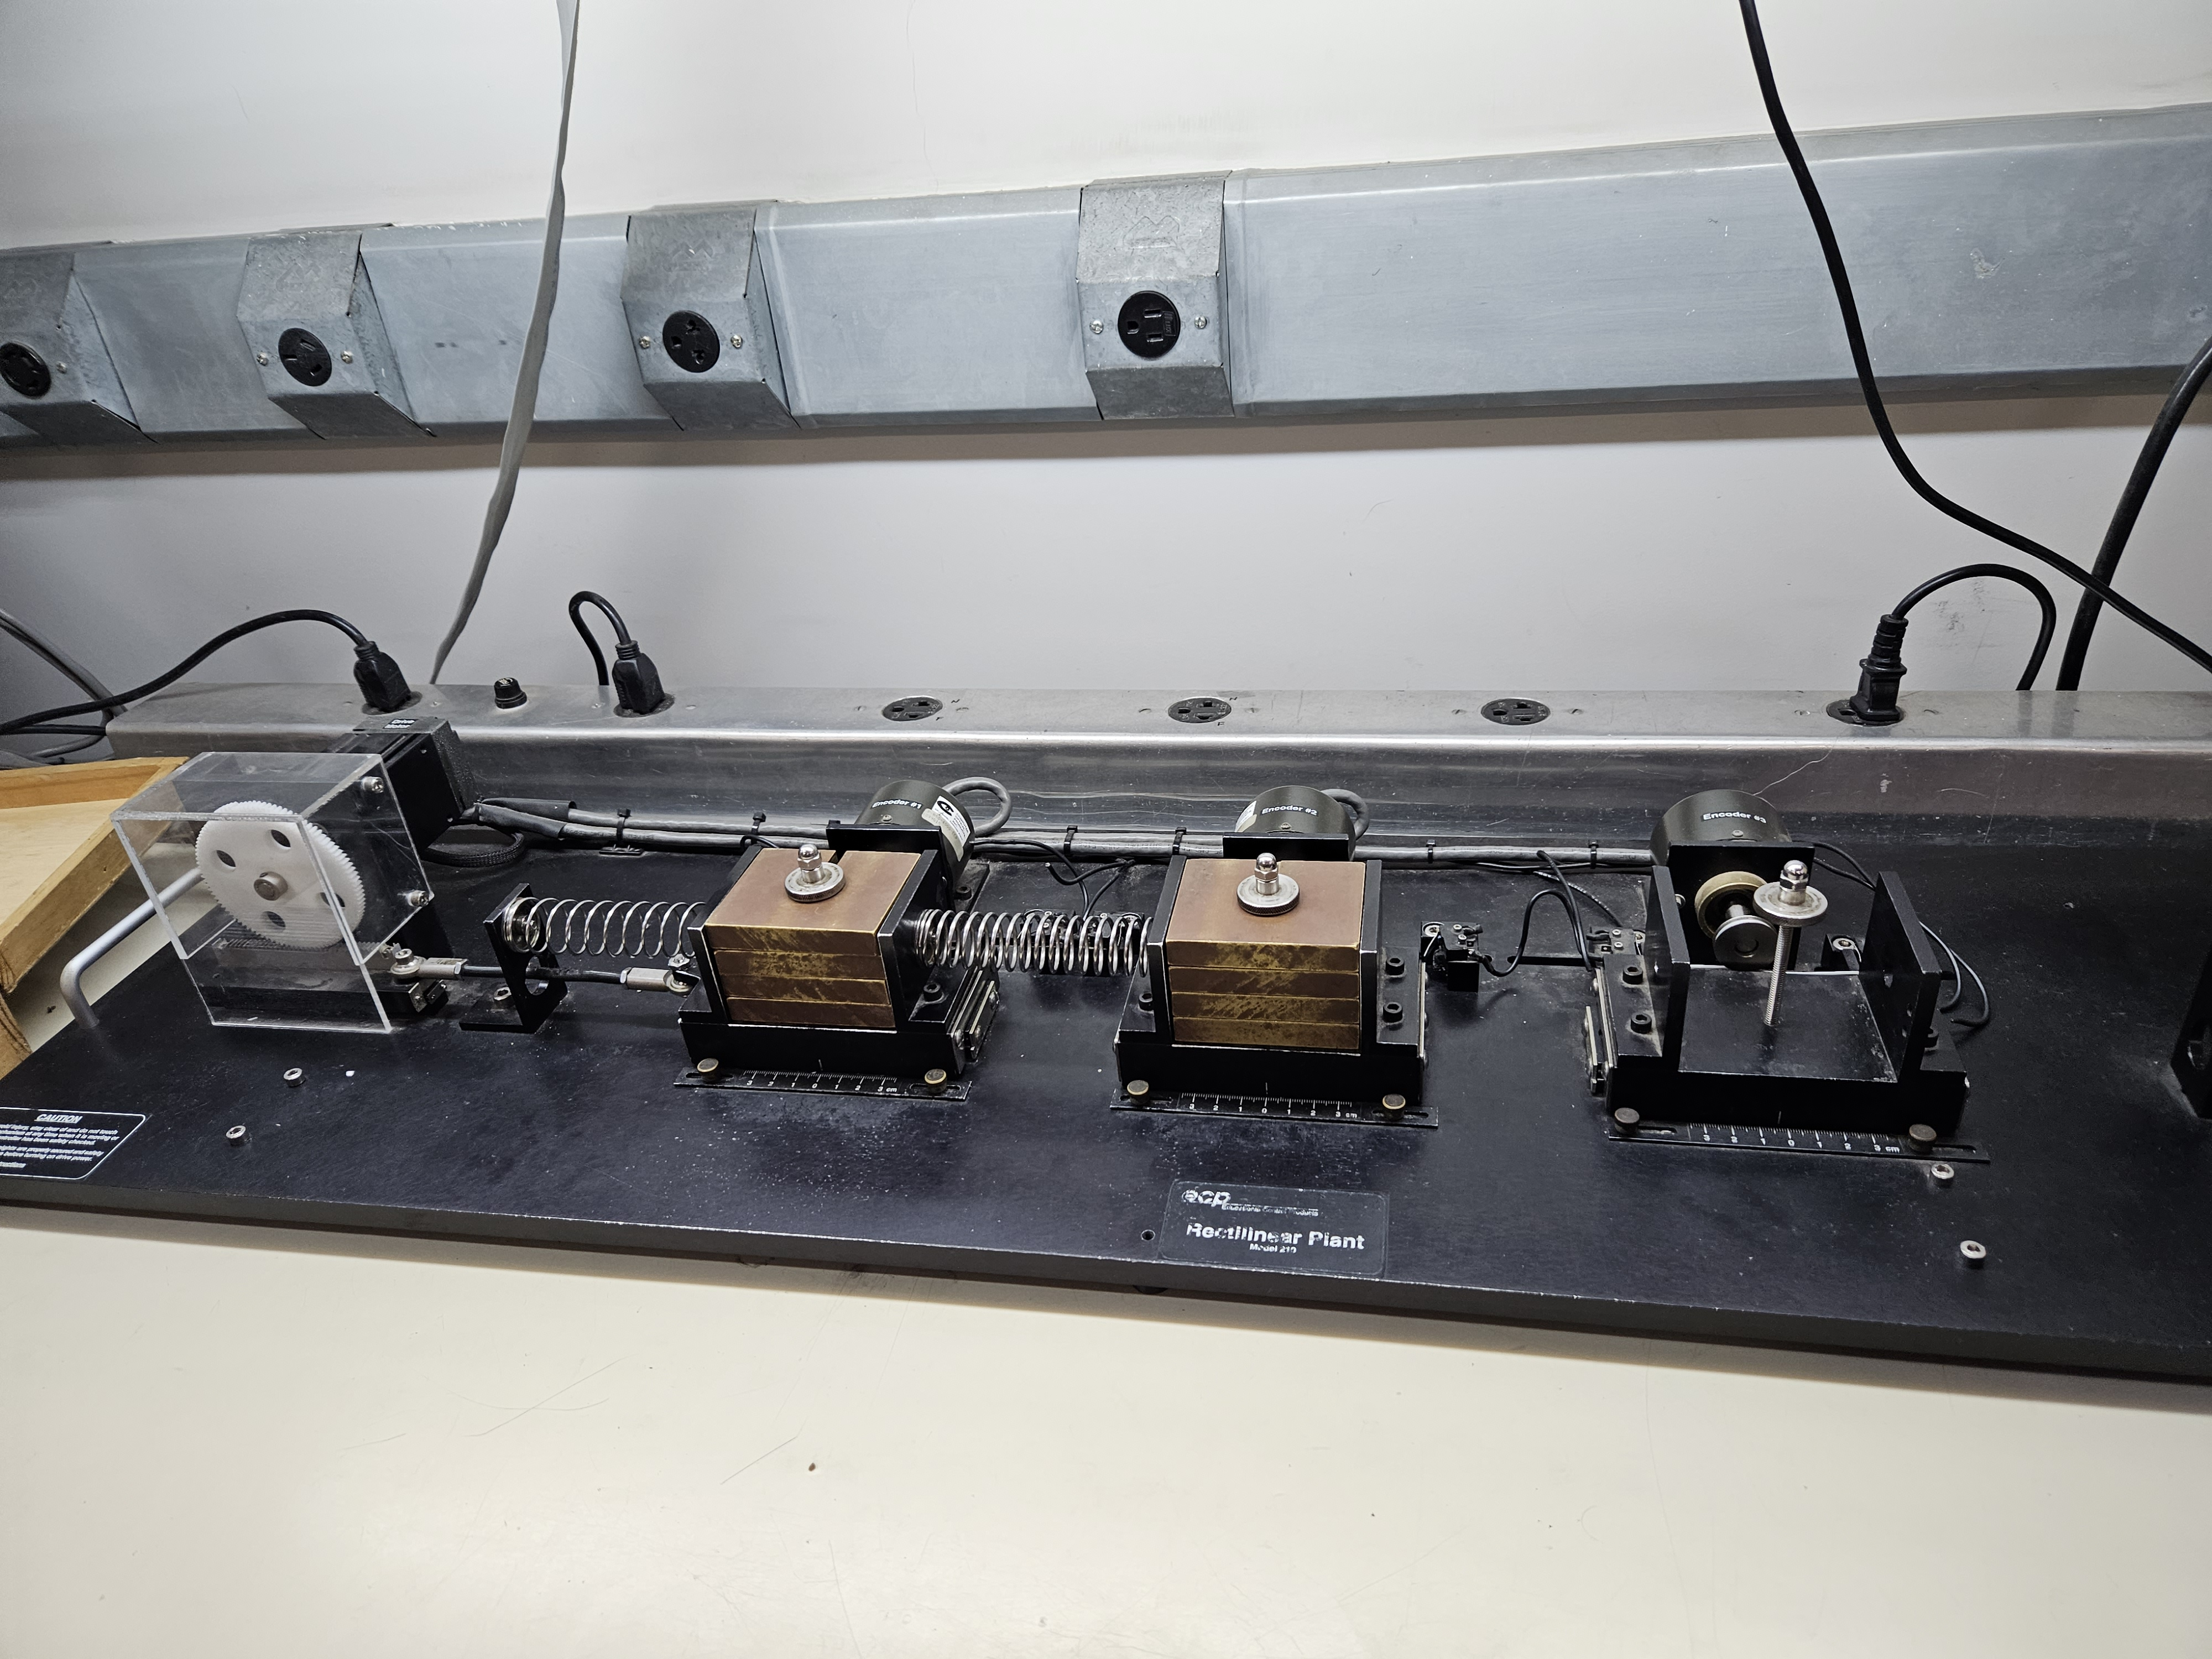
\includegraphics[width=8.4cm]{figures/planta_padrao.jpg}    % The printed column width is 8.4 cm.
  \caption{Figura da planta real estudada, composta por duas molas de diferentes coeficientes e massas de 500 gramas cada. Fonte: Autoral} 
  \label{fig:planta_padrao}
  \end{center}
\end{figure}

Com isso, nas seções subsequentes, exploraremos em detalhes a modelagem matemática do sistema
massa-mola, bem como o fundamento do controle utilizado e demonstrações práticas.

\section{Descrição da planta e especificação do desempenho desejado}

O controle a ser realizado visa, inicialmente, controlar a posição do segundo carrinho bem como tornar o sistema estável, erro nulo para entrada de degrau, 
tempo de acomodação menor do que 4 segundos e sobressinal até 20\%.

\section{Modelagem matemática e validação do modelo}



\subsection{Modelagem matemática}

Após a definição do sistema em espaço de estados, deve-se encontrar os parâmetros
$k1$, $k2$, $c1$, $c2$, $m1$ e $m2$. Para isso, analisa-se um sistema simples com um carro, um coeficiente de atrito e uma mola,
cuja equação característica é representada por:
\begin{equation}
  s^2 + \frac{c}{m}s + \frac{k}{m} = 0
\end{equation}
Esse é um sistema de segunda ordem, que é representado tipicamente por:
\begin{equation}
  s^2 + 2\omega_n \zeta s + \omega_n^2 = 0
\end{equation}
onde a frequência natural $\omega_n$ e o amortecimento $\zeta$ podem ser
encontrados facilmente através de respostas ao degrau.
Comparando os termos de ambas equações, tem-se:
\begin{equation}
  \label{eq:termo1}
  \frac{c}{m} = 2\omega_n \zeta
\end{equation}
\begin{equation}
  \label{eq:termo2}
  \frac{k}{m} = \omega_n^2
\end{equation}
Sendo assim, tem-se duas equações e três variáveis. Portanto, foram realizados quatro testes aplicados a duas diferentes partes da planta.
Dois testes são realizados com a mola $k1$ e o carro de massa $m1$, onde o primeiro teste consistiu na aplicação de um degrau de 2,5 cm
na entrada, com uma massa adicional de 2 kg sobre o carro. O segundo, por sua vez, consistiu na aplicação do mesmo degrau, mas sem a massa
adicional sobre o carro. Do primeiro teste, obtém-se $\omega_{n1}$ e $\zeta_1$, já do segundo, obtém-se $\omega_{n2}$ e $\zeta_2$.
O mesmos testes são realizados sobre a mola $k_2$ conectado ao carro de massa $m_2$ a fim de obter $\omega_{n3}$, $\zeta_3$ $\omega_{n4}$ e $\zeta_4$.
Pelas respostas ao degrau, a frequência natural pode ser encontrada calculando o período entre dos picos, o que se torna muito fácil com ajuda de uma calculadora.
O amortecimento pode ser encontrado analisando através da função $findpeaks$ do $MATLAB$ aplicado à resposta. Como as amplitudes dos picos caem exponencialmente através da relação
$e^{-\omega_n \zeta}$, seus valores foram submetidos a uma linearização através de um logaritmo
natural. O resultado da linearização é uma função de primeira ordem, onde o coeficiente angular é igual a $-\omega_n \zeta$.
Portanto, é possível obter o coeficiente de amortecimento através da frequência natural.
Com os valores do coeficiente de amortecimento e da frequência natural em mãos, o seguinte sistema de equações
pode ser resolvido para calcular os parâmetros dos testes 1 e 2, que foram submetidos na primeira parte da planta:
\begin{equation}
  \label{eq:sistema1}
  \left\{
\begin{array}{lr}
  \frac{c_1}{m_1 + 2} = 2\omega_{n1} \zeta_1 \\
  \frac{k_1}{m_1 + 2} = \omega_{n1}^2 \\
  \frac{k_1}{m_1} = \omega_{n2}^2
\end{array}
\right. 
\end{equation}
Os testes 3 e 4 foram submetidos na segunda parte da planta e, da mesma forma, que os testes 1 e 2, resultam no seguinte
sistema de equações:
\begin{equation}
  \label{eq:sistema21}
  \left\{
\begin{array}{lr}
  \frac{c_2}{m_2 + 2} = 2\omega_{n3} \zeta_3 \\
  \frac{k_2}{m_2 + 2} = \omega_{n3}^2 \\
  \frac{k_2}{m_2} = \omega_{n4}^2
\end{array}
\right. 
\end{equation}

\subsection{Testes 1 e 2}
Os gráficos das respostas ao degrau dos testes 1 e 2 estão presentes nas figuras \ref{fig:picos_teste_1} e \ref{fig:picos_teste_2}.
Os gráficos das amplitudes linearizadas sobre o tempo estão presentes nas figuras \ref{fig:regressao_teste_1} e \ref{fig:regressao_teste_2}.
\begin{figure}[!htb]
  \begin{center}
  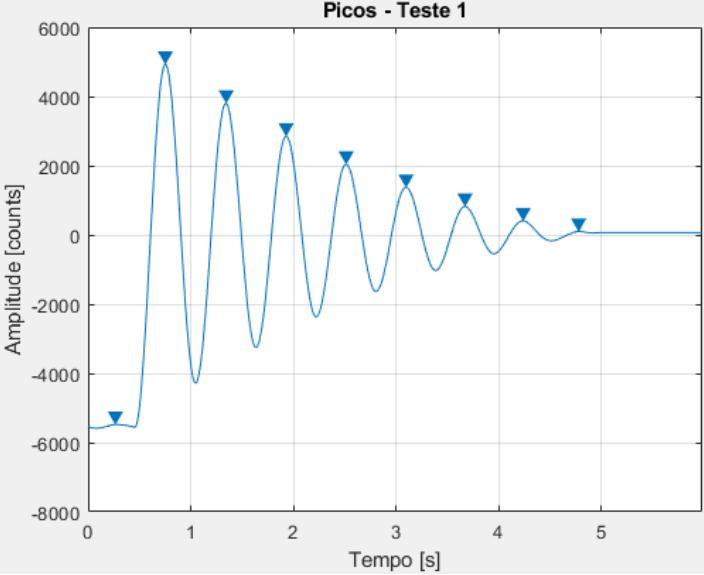
\includegraphics[width=8.4cm]{figures/picos_teste_1.png}    % The printed column width is 8.4 cm.
  \caption{Resposta ao degrau do teste 1. Fonte: Autoral.} 
  \label{fig:picos_teste_1}
  \end{center}
\end{figure}

\begin{figure}[!htb]
  \begin{center}
  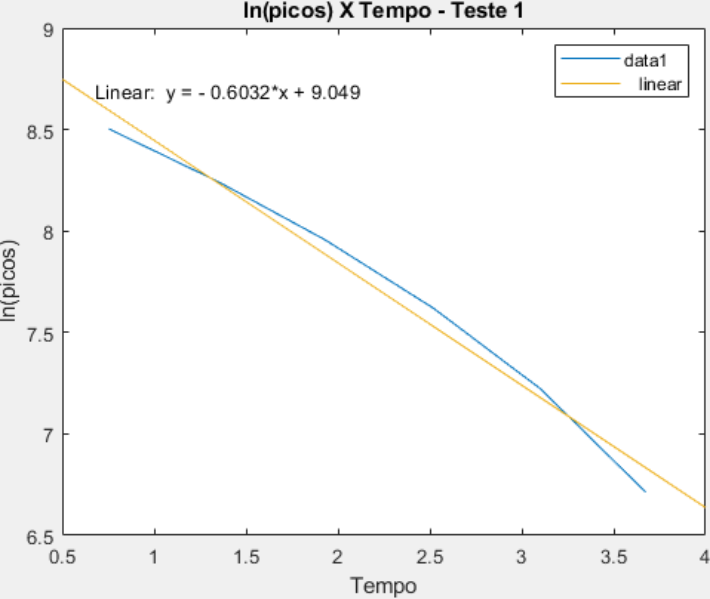
\includegraphics[width=8.4cm]{figures/regressao_teste_1.png}    % The printed column width is 8.4 cm.
  \caption{Amplitudes linearizadas do teste 1. Fonte: Autoral.} 
  \label{fig:regressao_teste_1}
  \end{center}
\end{figure}

\begin{figure}[!htb]
  \begin{center}
  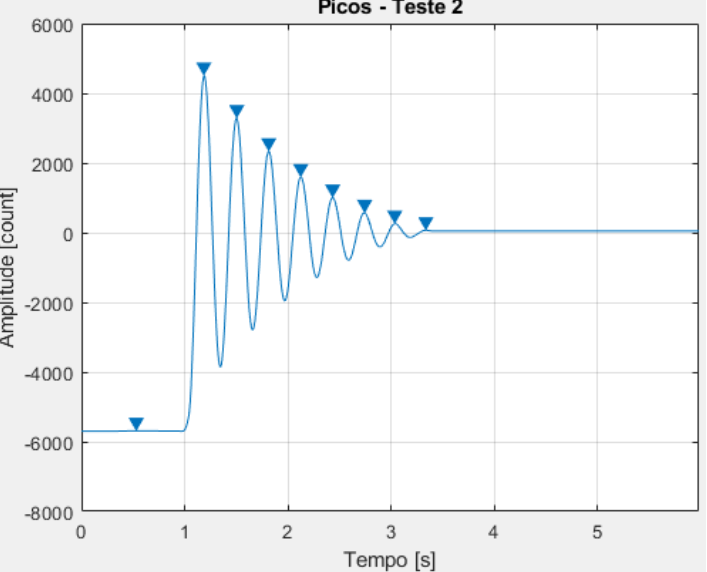
\includegraphics[width=8.4cm]{figures/picos_teste_2.png}    % The printed column width is 8.4 cm.
  \caption{Resposta ao degrau do teste 2. Fonte: Autoral.} 
  \label{fig:picos_teste_2}
  \end{center}
\end{figure}

\begin{figure}[!htb]
  \begin{center}
  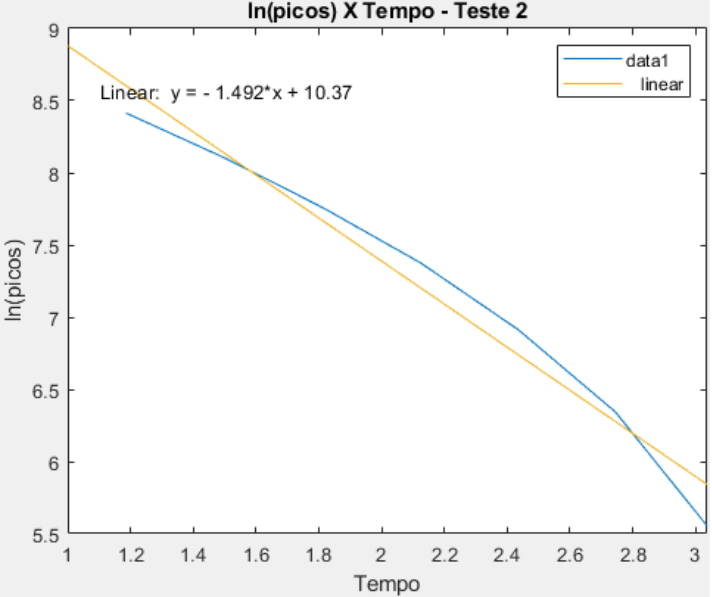
\includegraphics[width=8.4cm]{figures/regressao_teste_2.png}    % The printed column width is 8.4 cm.
  \caption{Amplitudes linearizadas do teste 2. Fonte: Autoral.} 
  \label{fig:regressao_teste_2}
  \end{center}
\end{figure}

Portanto, através dos gráficos da figura \ref{fig:picos_teste_1}, com ajuda do MATLAB, foi obtido uma frequência
natural de:
\begin{equation}
  \omega_{n1} = 10,5956
\end{equation}
O resultado da regressão linear da figura \ref{fig:regressao_teste_1} permite dizer que:
\begin{equation}
  0,6032 = \omega_{n1} \zeta_1  \rightarrow  \zeta_1 = \frac{0,6032}{\omega_{n1}} = 0,0569
\end{equation}
O mesmo procedimento foi feito com os resultados do teste 2, cujo resultados estão presentes nas figuras \ref{fig:picos_teste_2} e \ref{fig:regressao_teste_2}.
\begin{equation}
  \omega_{n2} = 19,6965
\end{equation}
\begin{equation}
  1,492 = \omega_{n2} \zeta_2  \rightarrow  \zeta_2 = \frac{1,492}{\omega_{n2}} = 0,0757
\end{equation}

Com os valores de $\omega_{n1}, \omega_{n2}, \zeta_1$ e $\zeta_2$ em mãos, é possível resolver o sistema \ref{eq:sistema1}
\begin{equation}
  \left\{
\begin{array}{lr}
  \frac{c_1}{m_1 + 2} = 2\omega_{n1} \zeta_1 \\
  \frac{k_1}{m_1 + 2} = \omega_{n1}^2 \\
  \frac{k_1}{m_1} = \omega_{n2}^2
\end{array}
\right.
\end{equation}

\begin{equation}
  \left\{
\begin{array}{lr}
  \frac{c_1}{m_1 + 2} = 2 \cdot 10,5956 \cdot 0,0569 \\
  \frac{k_1}{m_1 + 2} = 10,5956^2 \\
  \frac{k_1}{m_1} = 19,6965^2
\end{array}
\right.
\end{equation}

\begin{equation}
  \left\{
\begin{array}{lr}
  m_1 = 0,92 kg \\
  c_1 = 2,143 Ns/m \\
  k_1 = 356,5  N/m
\end{array}
\right.
\end{equation}
\subsection{Testes 3 e 4}

Após a aplicação do degrau de 2,5 cm ao sistema, a saída foi obtida e está presente na figura \ref{fig:picos_teste_3}.
Além disso, houve a linearização e regressão da amplitude dos picos da resposta ao degrau, assim como descrito nos testes anteriores,
e está presente na figura \ref{fig:regressao_teste_3}. Para o teste 4, a resposta ao degrau está presente na figura \ref{fig:picos_teste_4}
e a linearização dos picos juntamente da regressão linear está presente na figura \ref{fig:regressao_teste_4}.
\begin{figure}[!htb]
  \begin{center}
  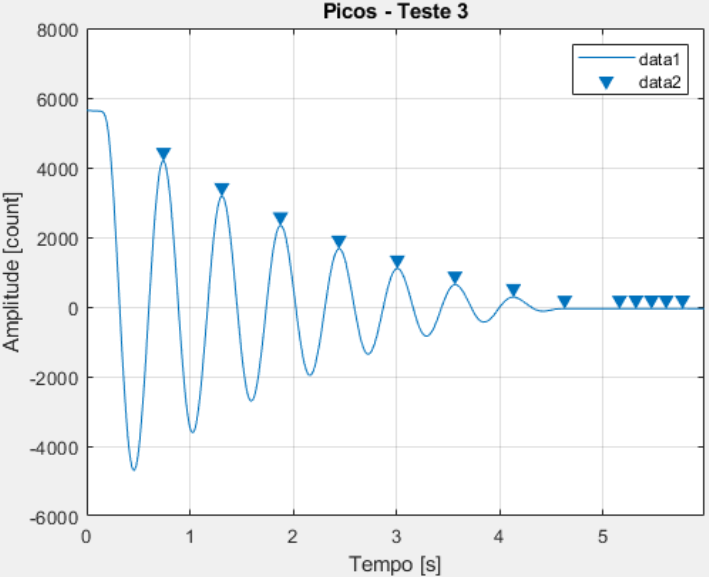
\includegraphics[width=8.4cm]{figures/picos_teste_3.png}    % The printed column width is 8.4 cm.
  \caption{Resposta ao degrau do teste 3. Fonte: Autoral.} 
  \label{fig:picos_teste_3}
  \end{center}
\end{figure}

\begin{figure}[!htb]
  \begin{center}
  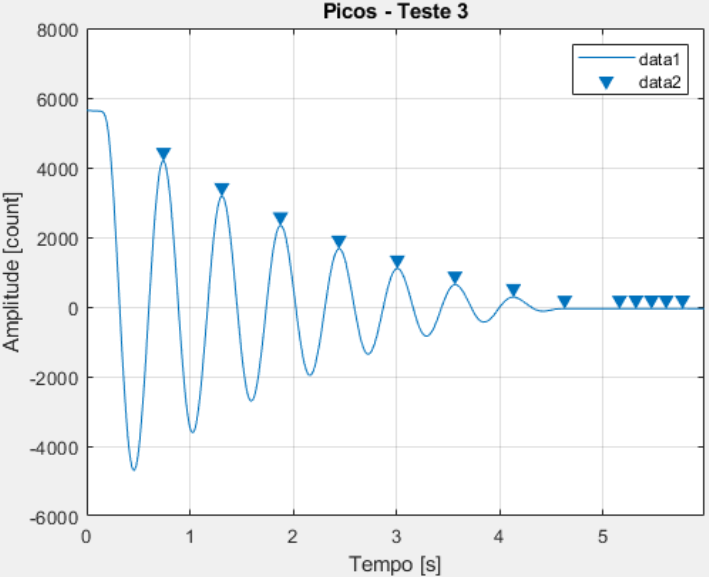
\includegraphics[width=8.4cm]{figures/picos_teste_3.png}    % The printed column width is 8.4 cm.
<<<<<<< HEAD
  \caption{Resposta ao degrau do teste 3. Fonte: Autoral.} 
  \label{fig:picos_teste_3}
=======
  \caption{Amplitudes linearizadas do teste 3. Fonte: Autoral.} 
  \label{fig:regressao_teste_3}
>>>>>>> c251b6a8f9a4fe7ced57a54468e7e8b951d61484
  \end{center}
\end{figure}

\begin{figure}[!htb]
  \begin{center}
  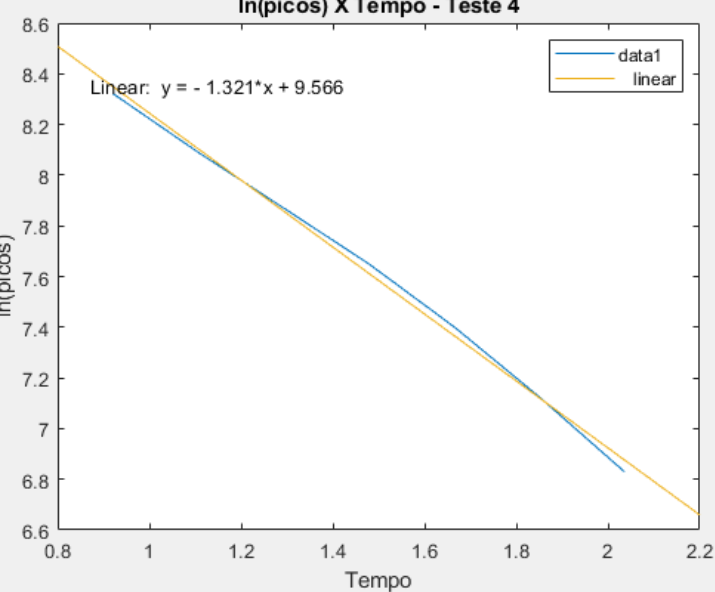
\includegraphics[width=8.4cm]{figures/regressao_teste_4.png}    % The printed column width is 8.4 cm.
<<<<<<< HEAD
  \caption{Amplitudes linearizadas do teste 4. Fonte: Autoral.} 
  \label{fig:regressao_teste_4}
=======
  \caption{Resposta ao degrau do teste 4. Fonte: Autoral.} 
  \label{fig:picos_teste_4}
>>>>>>> c251b6a8f9a4fe7ced57a54468e7e8b951d61484
  \end{center}
\end{figure}

\begin{figure}[!htb]
  \begin{center}
  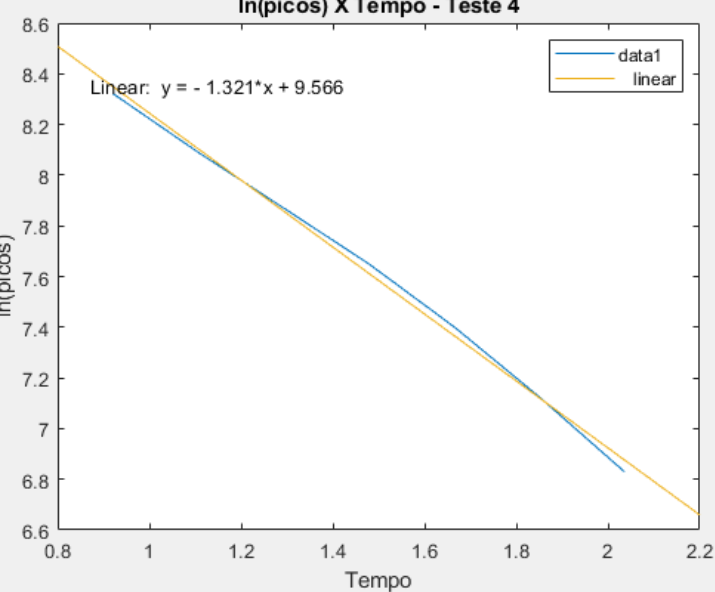
\includegraphics[width=8.4cm]{figures/regressao_teste_4.png}    % The printed column width is 8.4 cm.
  \caption{Amplitudes linearizadas do teste 4. Fonte: Autoral.} 
  \label{fig:regressao_teste_4}
  \end{center}
\end{figure}
Portanto, através da resposta ao degrau, obtém-se uma frequência natural de:
\begin{equation}
    \omega_{n3} = 11,1010
\end{equation}
Pela regressão linear, pode-se dizer que:
\begin{equation}
    \omega_{n3} \zeta_3 = 0,6515 \rightarrow \zeta_3 = \frac{0,6515}{\omega_{n3}} = 0,0587
\end{equation}

Realizando o mesmo procedimento para o teste 4, tem-se:
\begin{equation}
    \omega_{n4} = 33,7806
\end{equation}
Pela regressão linear, pode-se dizer que:
\begin{equation}
    \omega_{n4} \zeta_4 = 1,321 \rightarrow \zeta_4 = \frac{1,321}{\omega_{n4}} = 0,0391
\end{equation}

Aplicando os valores de frequência natural e amortecimento dos testes 3 e 4 ao sistema de equações \ref{eq:sistema2}, tem-se:

\begin{equation}
  \left\{
\begin{array}{lr}
  \frac{c_2}{m_2 + 2} = 2\omega_{n3} \zeta_3 \\
  \frac{k_1}{m_2 + 2} = \omega_{n3}^2 \\
  \frac{k_2}{m_2} = \omega_{n4}^2
\end{array}
\right.
\end{equation}

\begin{equation}
  \left\{
\begin{array}{lr}
  \frac{c_2}{m_2 + 2} = 2 \cdot 11,1010 \cdot 0,0587 \\
  \frac{k_2}{m_2 + 2} = 11,1010^2 \\
  \frac{k_2}{m_2} = 33,7806^2
\end{array}
\right.
\end{equation}

\begin{equation}
  \left\{
\begin{array}{lr}
  m_2 = 0,896 kg \\
  c_2 = 3,774 Ns/m \\
  k_2 = 1022,45 N/m
\end{array}
\right.
\end{equation}

\subsection{Validação do modelo}

Foi realizada a aplicação de uma entrada em degrau de tensão na planta em malha aberta, onde a sua resposta
foi comparada com a resposta ao degrau da planta simulada pelo $MATLAB$. Ambas as reposta apresentaram semelhanças,
o que é um bom sinal, haja vista as dificuldades enfrentadas até aqui.

\section{Projeto do controlador}

A principio, buscamos realizar o controlador proporcional, integrativo e derivativo (PID), 
por garantir erro nulo para entrada em degrau e por ser amplamente difundido nas industrias
e sistemas de controle em geral. A seguir será explicitado as tentativas para obter esse controlador.

\subsection{Primeira tentativa} %Falha obtida
Para obtenção dos parâmetros foi plotado o lugar das raizes da planta em malha fechada, figuras \ref{fig:lugar_raizes_mf} e \ref{fig:lugar_raizes_mf_aproximada}.
Com o lugar da raizes traçados, foi utilizado o \textit{sisotool} para realizar a escolha da localização dos polos e ganho do controlador PID, com isso realizamos
o cancelamento de polos mais instaveis, os polos localizados mais a direita do circulo unitário, e escolhemos um ganho arbritário para sair da instabilidade e obter
uma resposta satisfatória. Por fim, implementamos o controle na planta e visualizamos que a resposta obtida na planta não condizia com o esperado visto no \textit{MatLab},
independente da referência inserida, o carrinho não se mexia nada, consequentemente, acreditamos que o ganho do Kp estava baixo e fomos aumentando de forma empirica, 
após diversos aumentos no Kp, o carrinho começou a se mexer. Sendo assim, a planta modelada era equivalente com o sistema em malha aberta, mas em malha fechada o comportamento
era diferente. De forma a elucidar o ocorrido, assumimos de que a falha ocorreu devido aos coeficientes de atrito C1 e C2, portanto, aumentamos esses parâmetros, empiricamente, até
obter uma resposta satisfatória para iniciar novamente o processo de controle mas com uma nova modelagem da planta. 

\begin{figure}[!htb]
  \begin{center}
  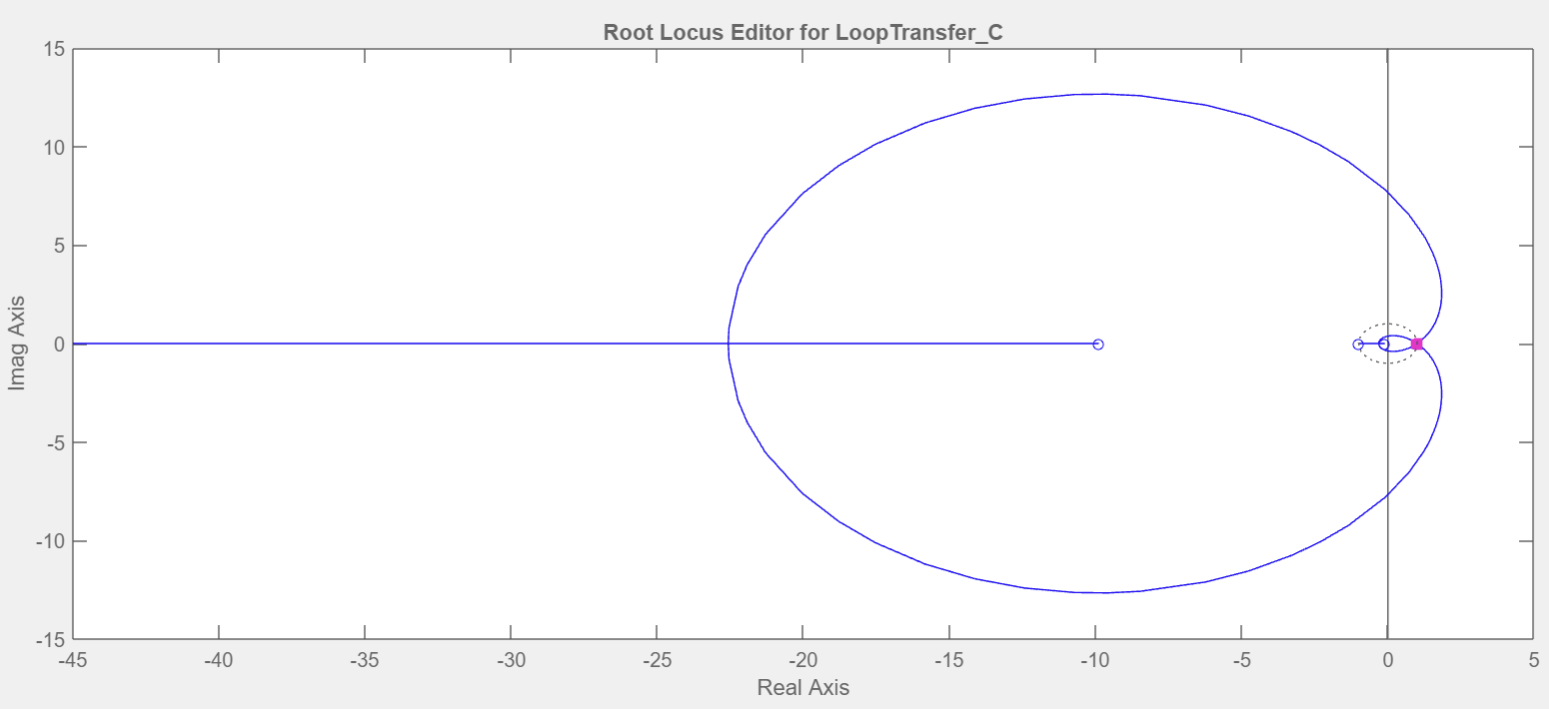
\includegraphics[width=8.4cm]{figures/lugar_raizes_mf.png}    % The printed column width is 8.4 cm.
  \caption{Lugar da raizes da malha fechada da planta. Fonte: autoral, produzida com \textit{matlab}.} 
  \label{fig:lugar_raizes_mf}
  \end{center}
\end{figure}

\begin{figure}[!htb]
  \begin{center}
  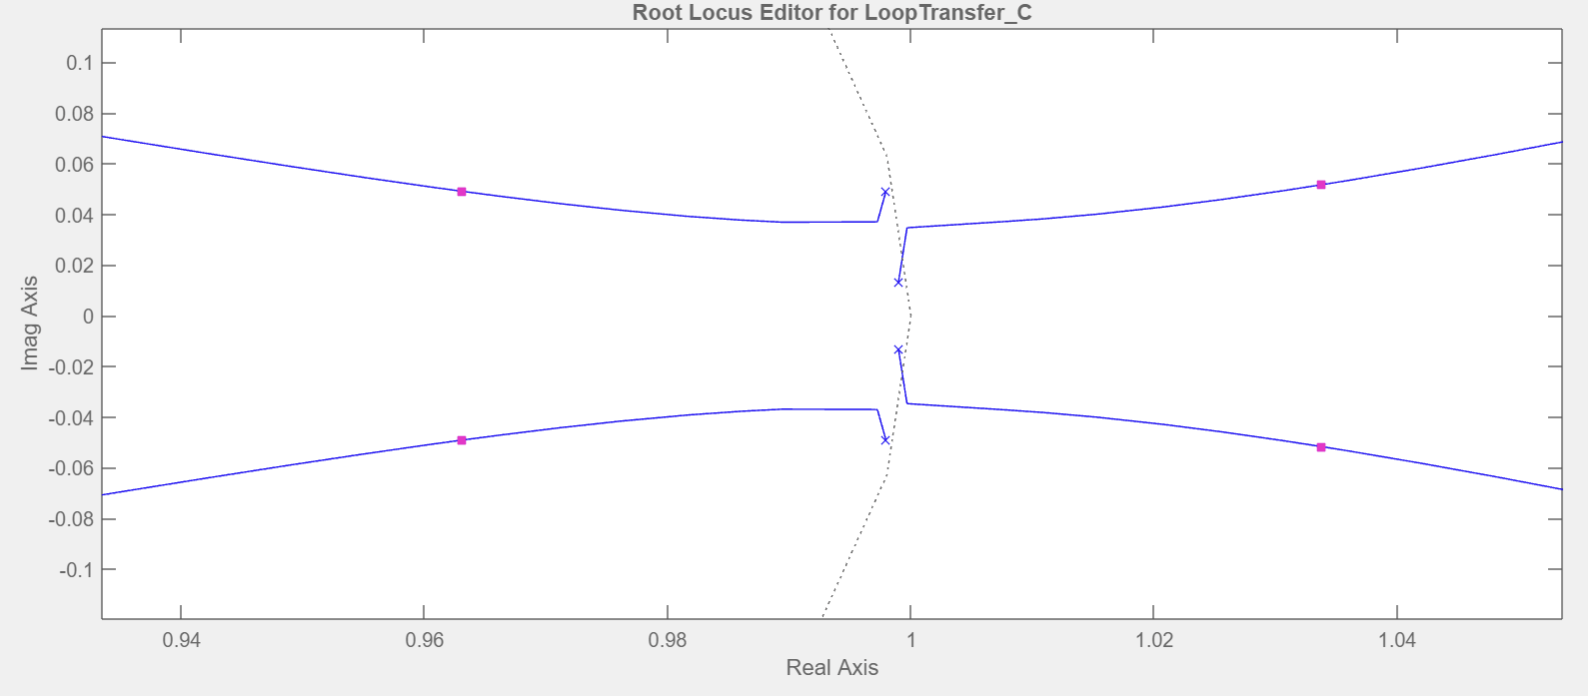
\includegraphics[width=8.4cm]{figures/lugar_raizes_mf_aproximada.png}    % The printed column width is 8.4 cm.
  \caption{Lugar da raizes da malha fechada da planta aproximada na extremidade do circulo unitário. Fonte: autoral, produzida com \textit{matlab}.} 
  \label{fig:lugar_raizes_mf_aproximada}
  \end{center}
\end{figure}

\subsection{Segunda tentiva} %Controle corrigido
Sequencialmente após a correção dos parâmetros C1 e C2, de forma impirica, recalculamos o modelo obtendo as seguintes
matrizes do espaço de estados:

Posteriormente foi realizado um novo estudo sobre o lugar das raizes em malha fechada, figura \ref{fig:lugar_raizes_mf_atualizada}, em que
aproximando para próximo da extremidade do circulo unitário temos a figura \ref{fig:lugar_raizes_mf_atualizada_zoom}. 
Em que é possível perceber que a caracteristica da resposta do modelo é fortemente marcada por dois pares de polos conjugados
próximos a extremidade do circulo unitário levando para a instabilidade do sistema, como mostra a resposta ao degrau do sistema, figura \ref{fig:resposta_Degrau_mf_atualizada}.

\begin{figure}[!htb]
  \begin{center}
  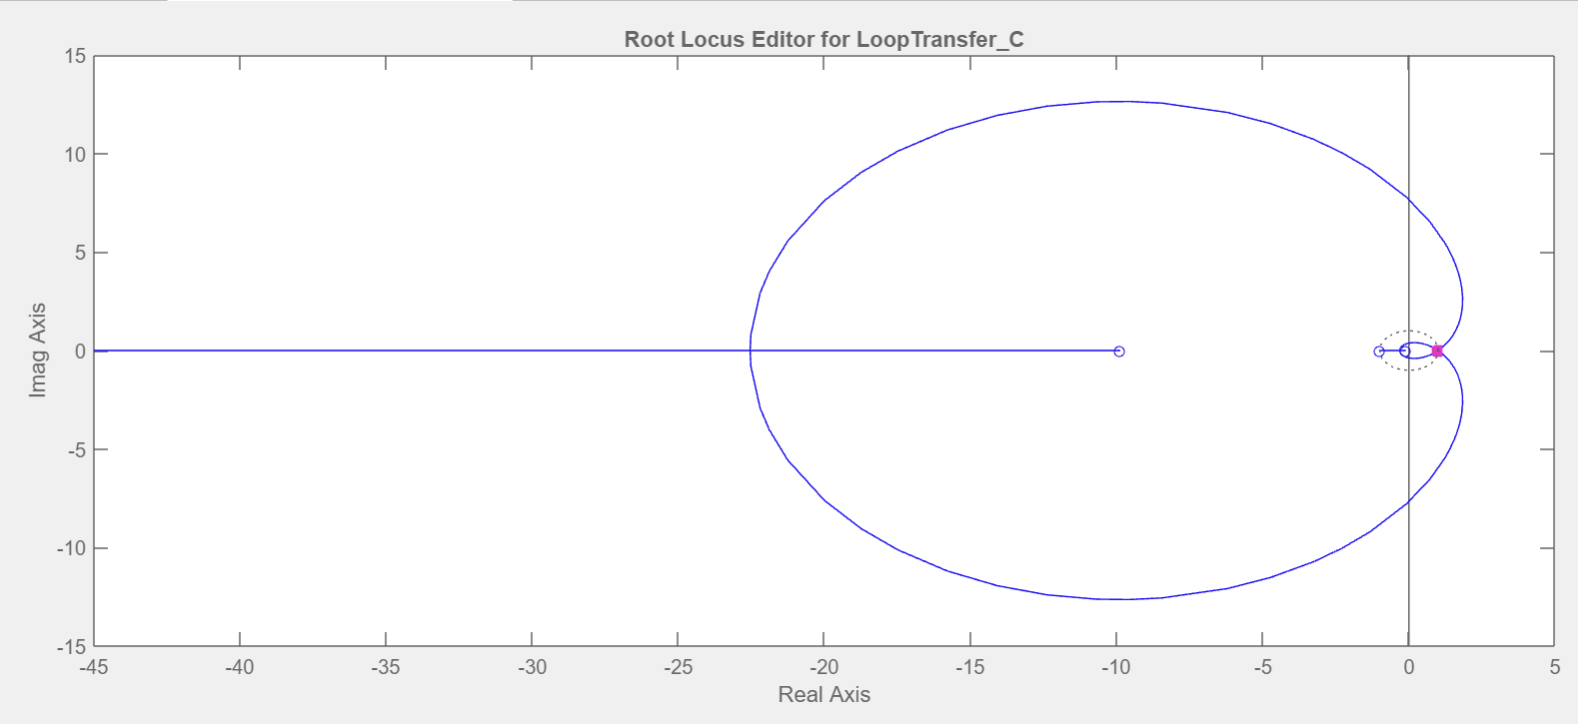
\includegraphics[width=8.4cm]{figures/lugar_raizes_mf_corrigida.png}    % The printed column width is 8.4 cm.
  \caption{Lugar da raizes da malha fechada da planta atualizada. Fonte: autoral, produzida com \textit{matlab}.} 
  \label{fig:lugar_raizes_mf_atualizada}
  \end{center}
\end{figure}

\begin{figure}[!htb]
  \begin{center}
  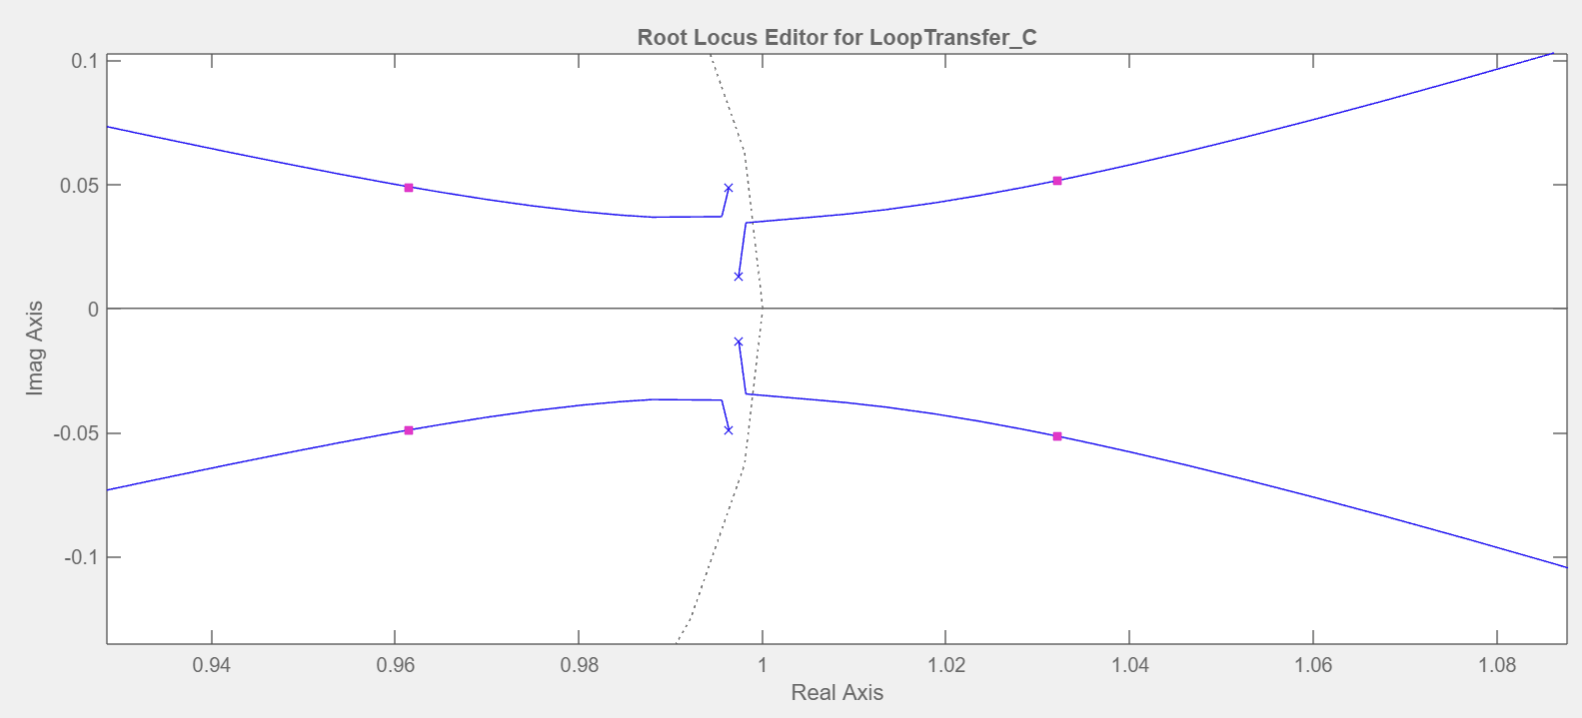
\includegraphics[width=8.4cm]{figures/lugar_raizes_mf_corrigida_aproximada.png}    % The printed column width is 8.4 cm.
  \caption{Lugar da raizes da malha fechada da planta atualizada aproximada na extremidade do circulo unitário. Fonte: autoral, produzida com \textit{matlab}.} 
  \label{fig:lugar_raizes_mf_atualizada_zoom}
  \end{center}
\end{figure}

\begin{figure}[!htb]
  \begin{center}
  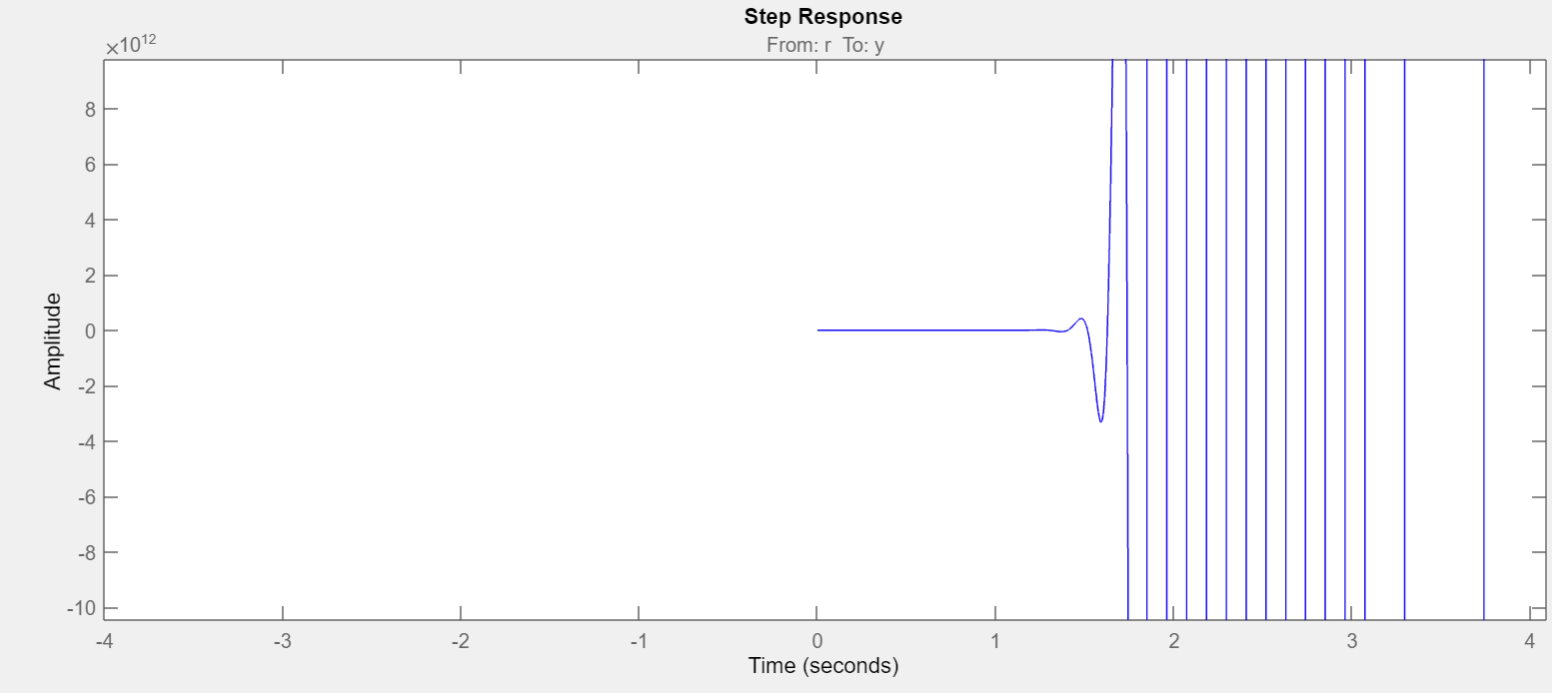
\includegraphics[width=8.4cm]{figures/resposta_degrau_mf_atualizado.png}    % The printed column width is 8.4 cm.
  \caption{Resposta ao degrau da planta atualizada, sem controlador, indo para a instabilidade. Fonte: autoral, produzida com \textit{matlab}.} 
  \label{fig:resposta_Degrau_mf_atualizada}
  \end{center}
\end{figure}

Com isso, foi inserido o integrador e um par de zeros conjugados, controlador PID, próximo ao par de polos conjugados mais a direita do circulo unitário com 
a finalidade de atraí-los para dentro do circulo unitário, estabilizando o sistema e melhorando a margem de ganho. Nesse processo visualizamos
que o integrador colocado fazia com que o lugar das raizes do segundo par de polos conjugados da planta direcionasse para a instabilidade, portanto,
procuramos alocar o par de zeros conjugados de forma a garantir a não instabilidade do primeiro par de polos e de aumentar a margem de ganho em relação
ao segundo par de polos, para tal, o par de zeros deveria se localizar entre ambos os polos, mas mais próximo do primeiro. O lugar das raizes do controlador
é explicitado pelas figuras \ref{fig:lugar_raizes_mf_atualizada_controlador} e \ref{fig:lugar_raizes_mf_atualizada_controlador_zoom}. 

\begin{figure}[!htb]
  \begin{center}
  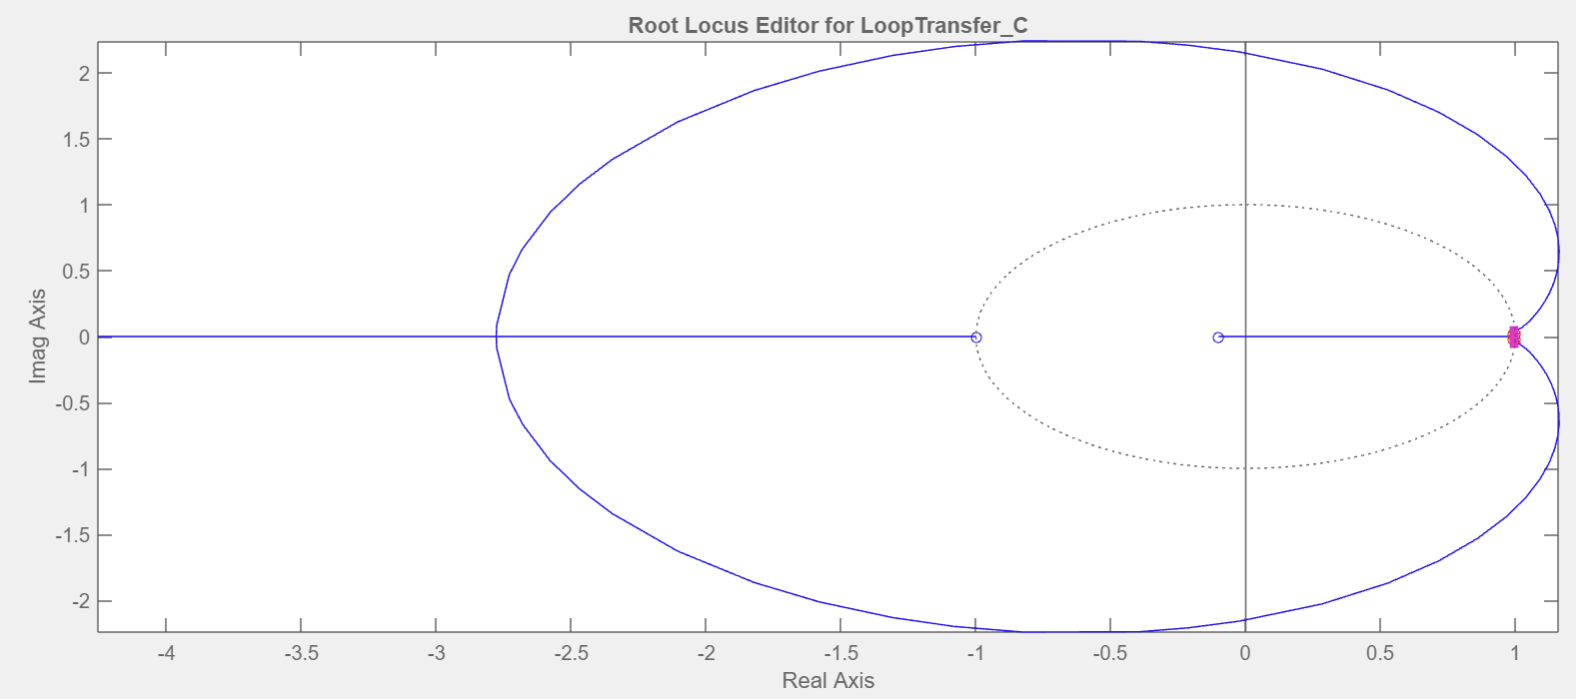
\includegraphics[width=8.4cm]{figures/lugar_raizes_controlador_finalpng.png}    % The printed column width is 8.4 cm.
  \caption{Lugar da raizes da malha fechada da planta atualizada com controlador PID. Fonte: autoral, produzida com \textit{matlab}.} 
  \label{fig:lugar_raizes_mf_atualizada_controlador}
  \end{center}
\end{figure}


\begin{figure}[!htb]
  \begin{center}
  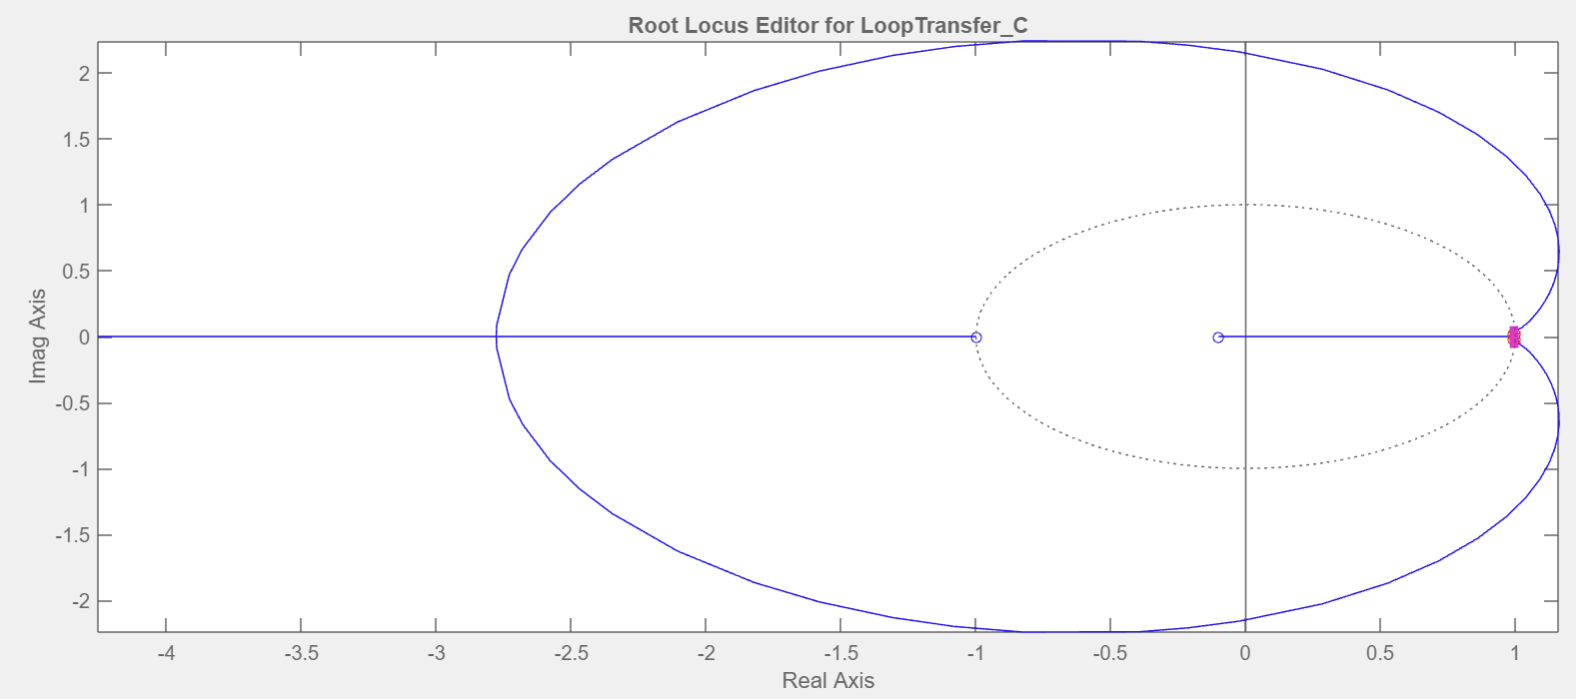
\includegraphics[width=8.4cm]{figures/lugar_raizes_controlador_finalpng.png}    % The printed column width is 8.4 cm.
  \caption{Lugar da raizes da malha fechada da planta atualizada com controlador PID aproximada na extremidade do circulo unitário. Fonte: autoral, produzida com \textit{matlab}.} 
  \label{fig:lugar_raizes_mf_atualizada_controlador_zoom}
  \end{center}
\end{figure}

Posteriormente, foi ajustado o ganho do controlador visualizando a resposta ao degrau do sistema com controlador, tendo como foco que o tempo de acomodação
fosse menor do que 4 segundos e principalmente que não houvesse sobressinal, pois como a planta possui uma margem de apenas 3 centimetros, sendo que nos 3 centimetros
possui uma chave fim de curso em que corta a alimentação do motor, o sobressinal atrapalha muito o controle, a reposta ao degrau obtida é representada pela curva 'Modelado' na figura \ref{fig:comparacao_mf_controle_step}.
Por fim, a equação do controlador PID obtido está explicitada na equação \ref{eq:controlador}.

\begin{equation}
  C = \frac{0,27951(z^2 - 1,994z + 0,9948)}{(z-1)}
  \label{eq:controlador}
\end{equation}

% Retirei essa figura para poder diminuir no espaço, uma vez q essa curva está dentro de outro gráfico
%\begin{figure}[!htb]
%  \begin{center}
%  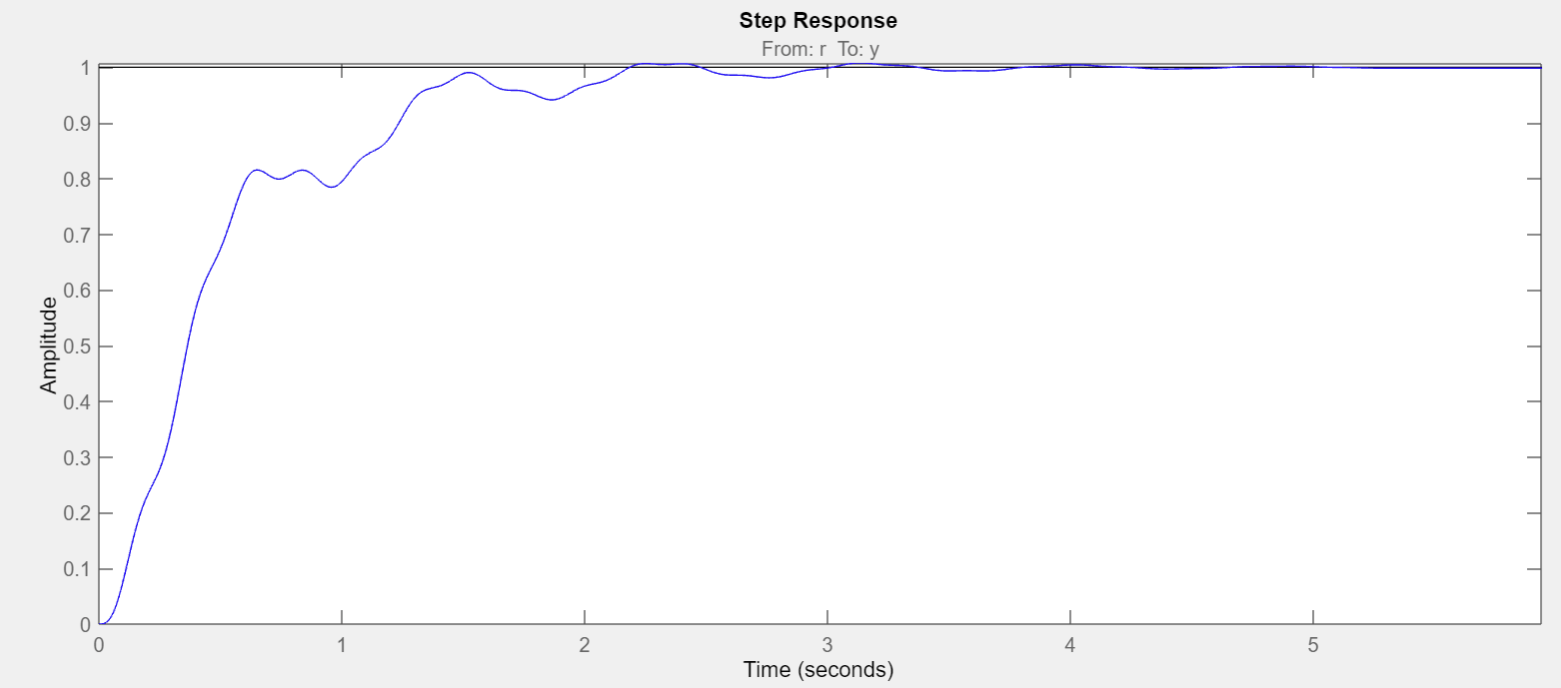
\includegraphics[width=8.4cm]{figures/resposta_degrau_controlador_final.png}    % The printed column width is 8.4 cm.
%  \caption{Resposta ao degrau da malha fechada da planta atualizada com controlador PID. Fonte: autoral, produzida com \textit{matlab}.} 
%  \label{fig:resposta_degrau_mf_atualizado_controlador}
%  \end{center}
%\end{figure}

No final, o controlador foi implementado e aplicado um degrau unitário na planta com o objetivo de comparar o resultado real com o esperado
pela modelagem, essa comparação é representada pela figura \ref{fig:comparacao_mf_controle_step}.

\begin{figure}[!htb]
  \begin{center}
  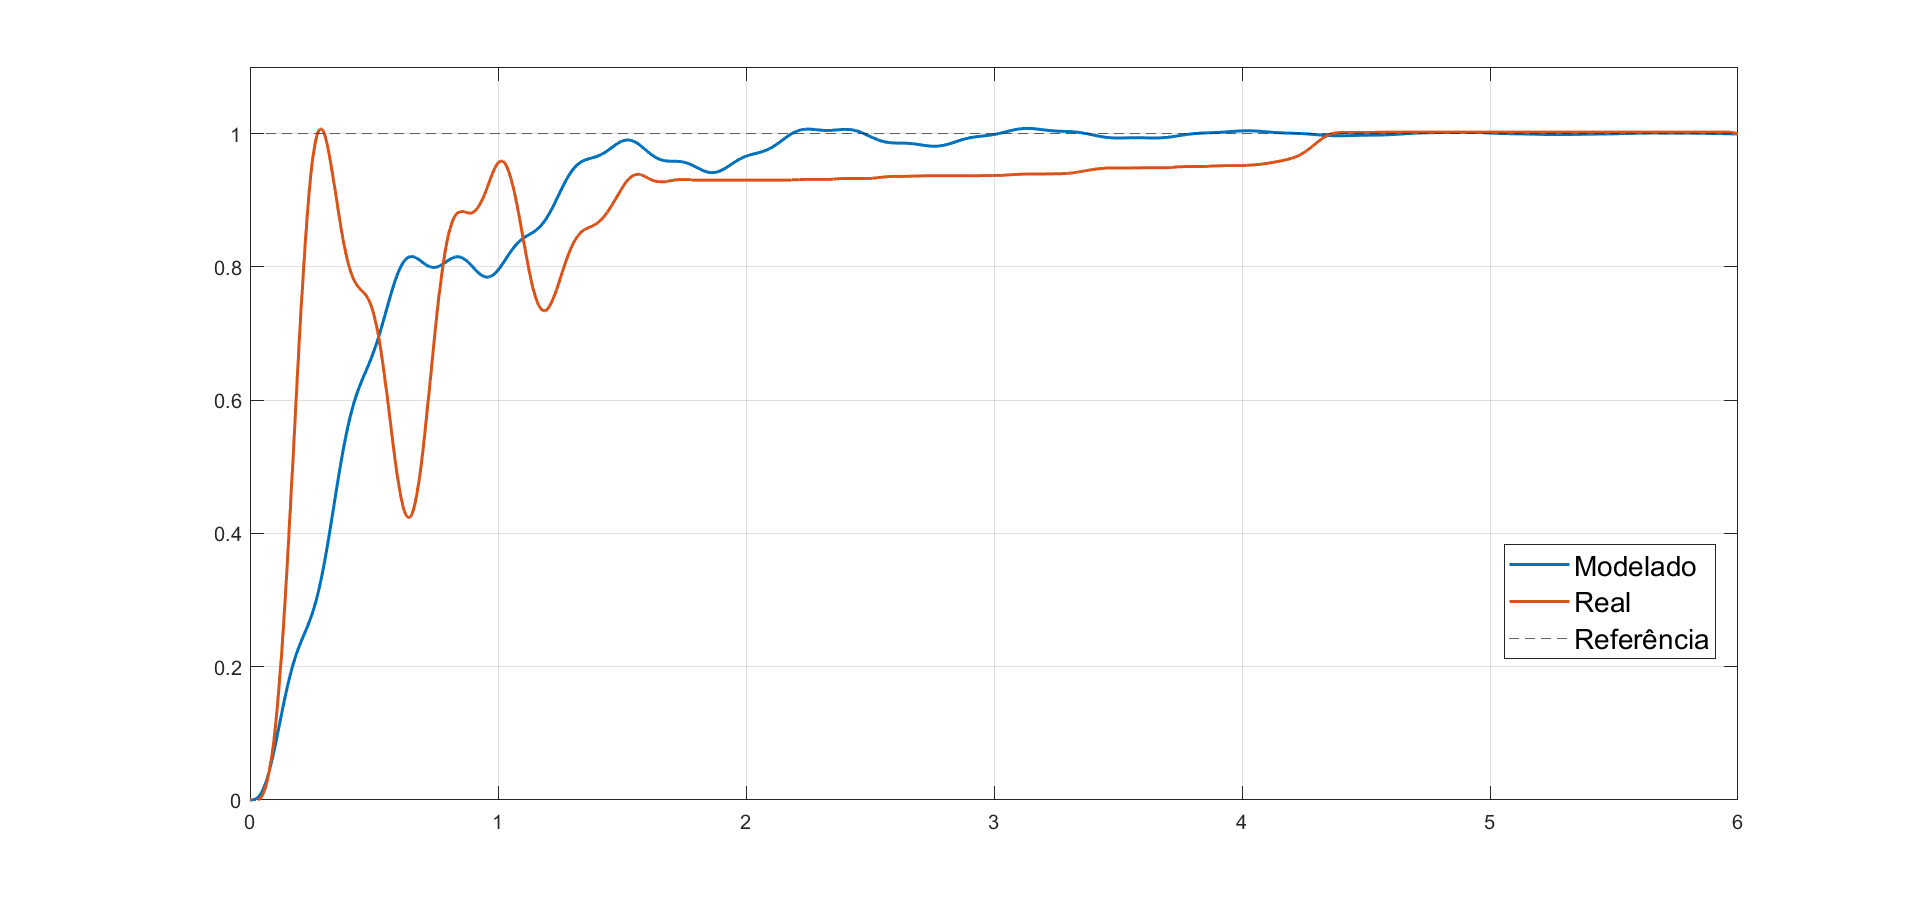
\includegraphics[width=8.4cm]{figures/comparacao_mf_controle_step.png}    % The printed column width is 8.4 cm.
  \caption{Comparação da resposta ao degrau em MF da planta em relação ao modelo, com controlador PID. Fonte: autoral, produzida com \textit{matlab}.} 
  \label{fig:comparacao_mf_controle_step}
  \end{center}
\end{figure}

Nessa comparação é possível perceber uma dinâmica aproximada entre os modelos, todavia, há algumas divergências nas amplitudes do movimento do período transitório
e demora para estabilização no regime permanente.  

\section{Resultados experimentais em malha fechada}

Essa seção testa o controle obtido em diversas situações e entradas diferentes na planta.

% Coloquei esse gráfico dentro da parte de controle comparando com o modelo
%\begin{figure}[!htb]
%  \begin{center}
%  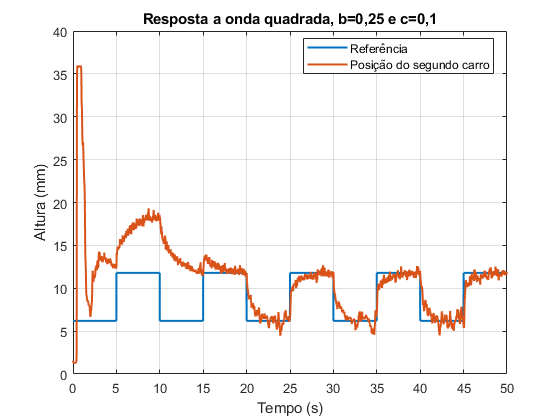
\includegraphics[width=8.4cm]{figures/resultado_teste4.png}    % The printed column width is 8.4 cm.
%  \caption{Resposta ao degrau unitário da planta, carro 1 e 2 com 4 pesos. Fonte: autoral, produzido com \textit{matlab} por meio dos dados coletados na planta.} 
%  \label{fig:teste_step1_c1_4p_c2_4p}
%  \end{center}
%\end{figure}

\begin{figure}[!htb]
  \begin{center}
  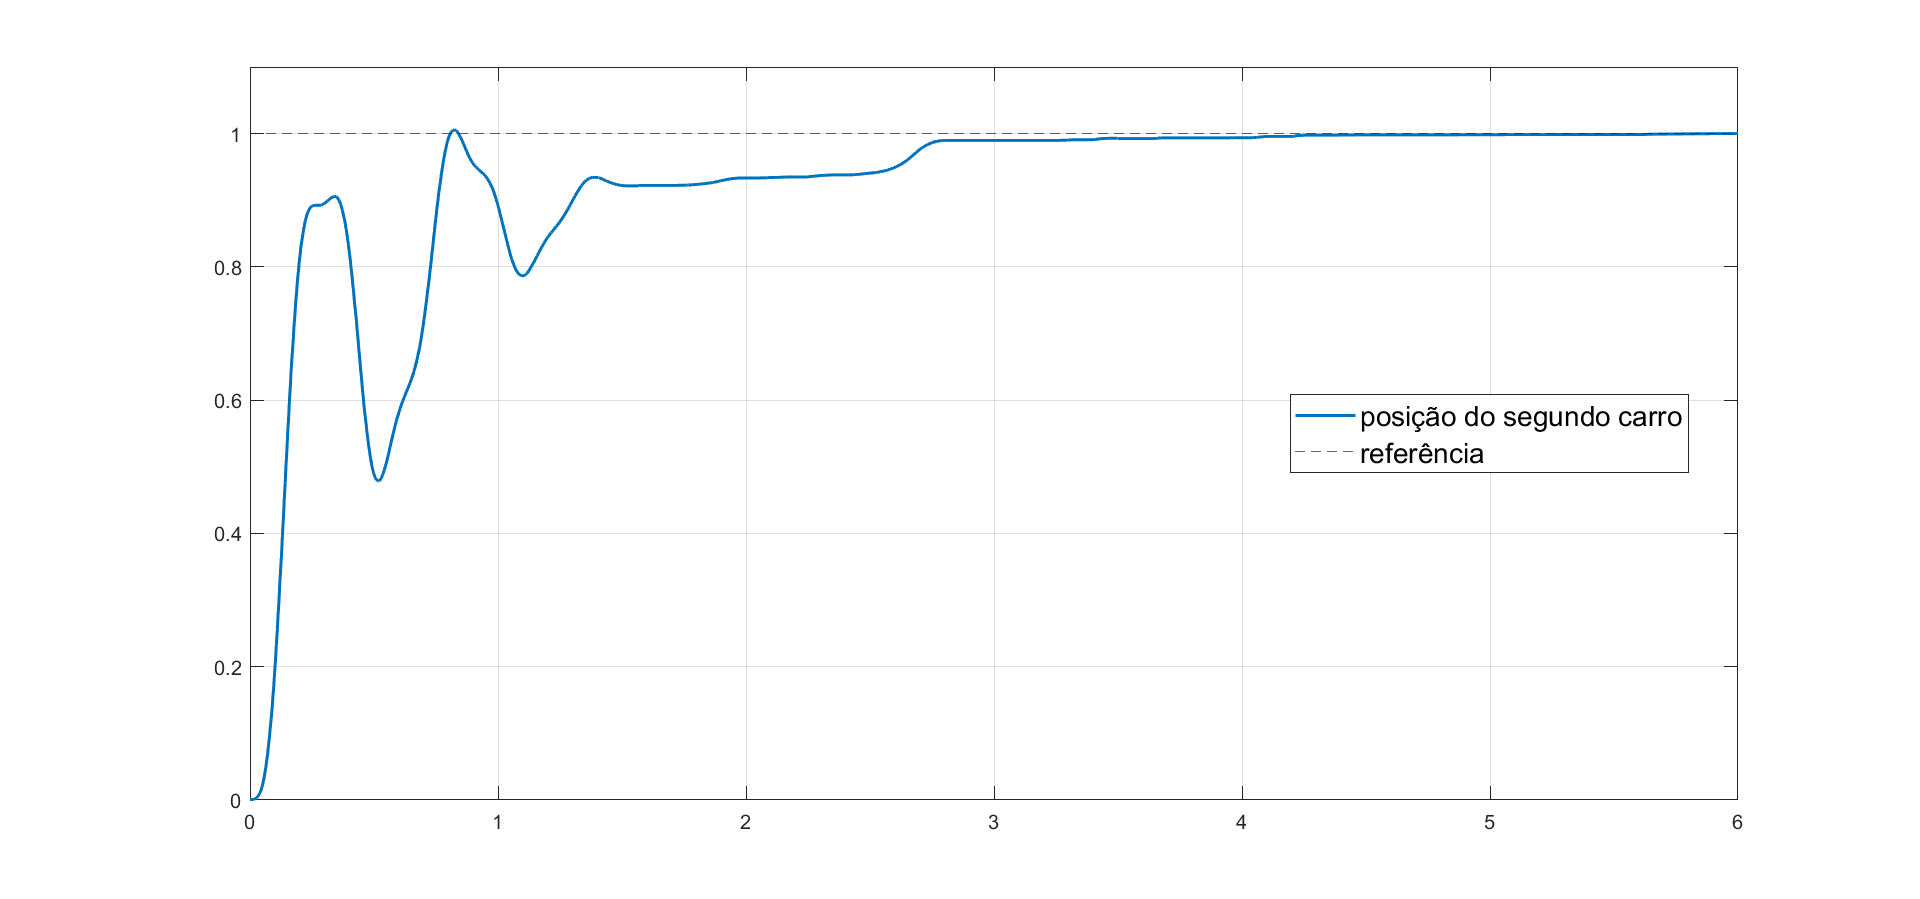
\includegraphics[width=8.4cm]{figures/resultado_teste1.png}    % The printed column width is 8.4 cm.
  \caption{Resposta ao degrau unitário da planta, carro 1 com 1 peso e carro 2 com 4 pesos. Fonte: autoral, produzido com \textit{matlab} por meio dos dados coletados na planta.} 
  \label{fig:teste_step1_c1_1p_c2_4p}
  \end{center}
\end{figure}

\begin{figure}[!htb]
  \begin{center}
  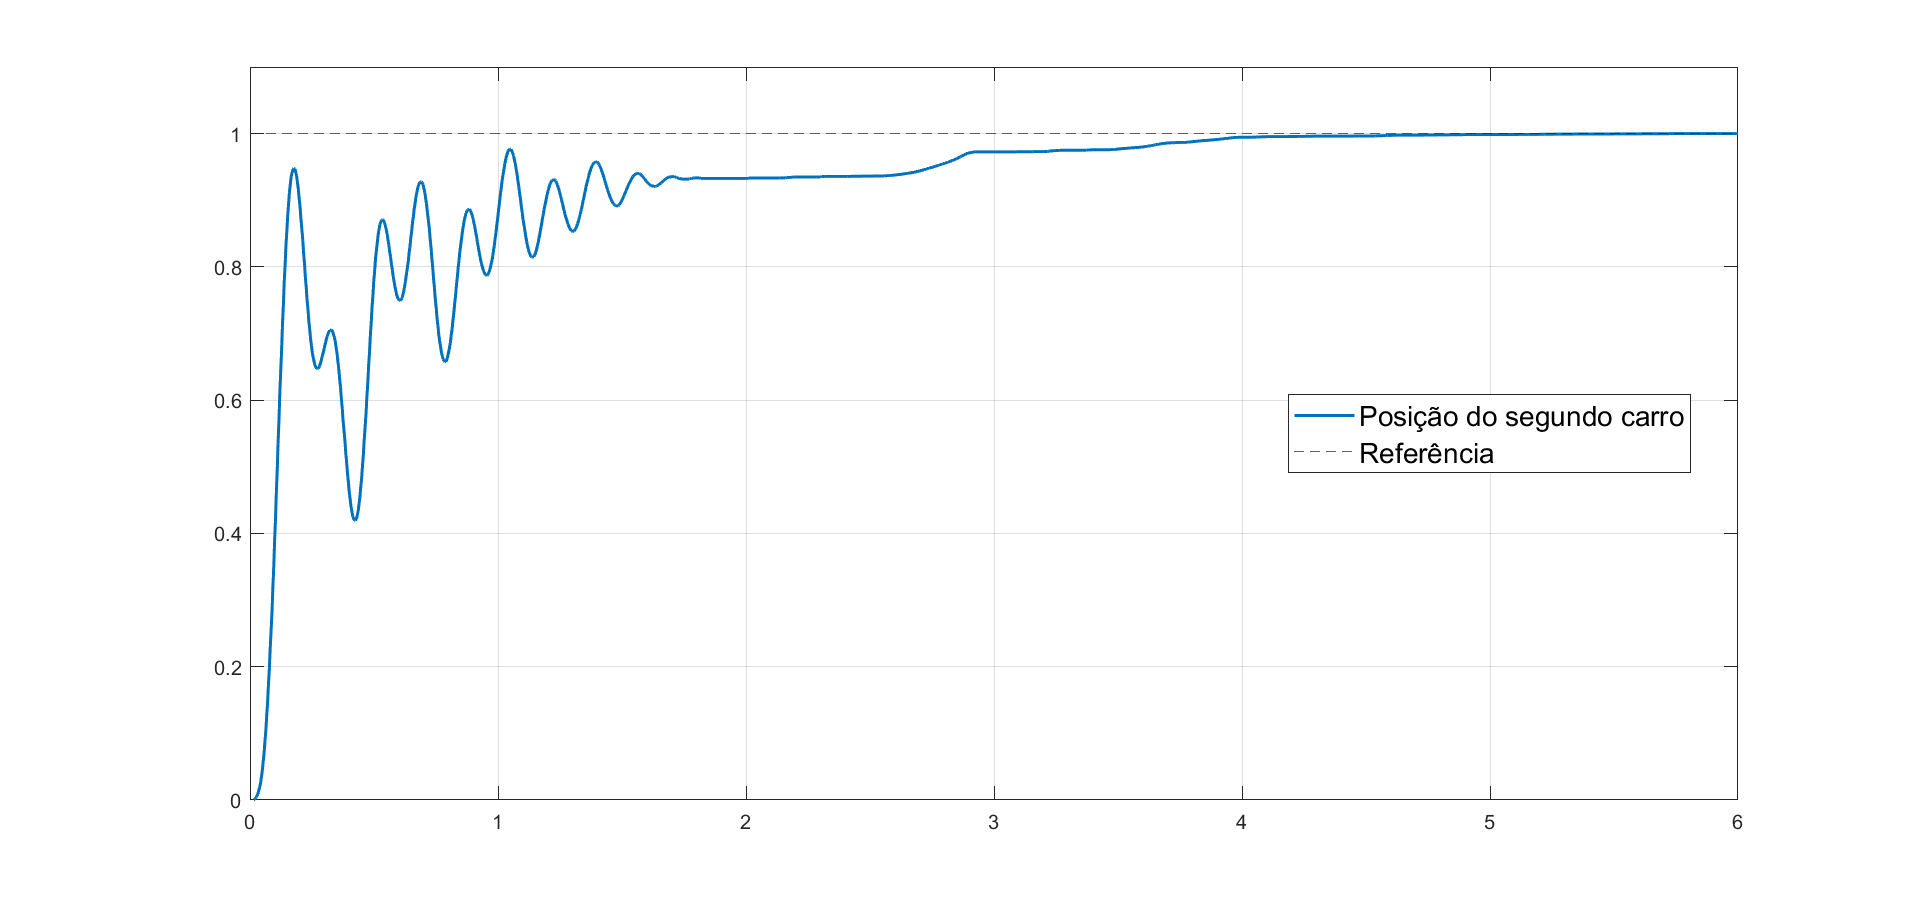
\includegraphics[width=8.4cm]{figures/resultado_teste2.png}    % The printed column width is 8.4 cm.
  \caption{Resposta ao degrau unitário da planta, carro 1 e 2 com 1 peso. Fonte: autoral, produzido com \textit{matlab} por meio dos dados coletados na planta.} 
  \label{fig:teste_step1_c1_1p_c2_1p}
  \end{center}
\end{figure}

\begin{figure}[!htb]
  \begin{center}
  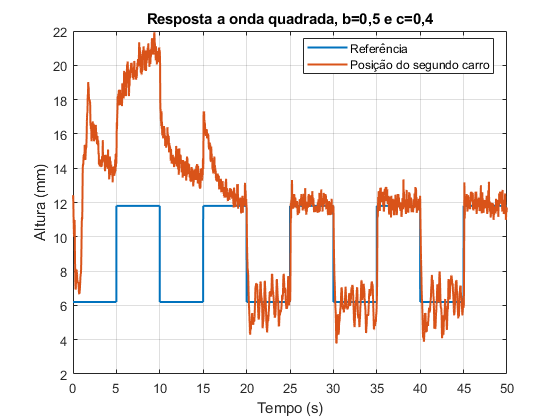
\includegraphics[width=8.4cm]{figures/resultado_teste3.png}    % The printed column width is 8.4 cm.
  \caption{Resposta ao degrau unitário da planta, carro 1 e 2 com nenhum peso. Fonte: autoral, produzido com \textit{matlab} por meio dos dados coletados na planta.} 
  \label{fig:teste_step1_c1_0p_c2_0p}
  \end{center}
\end{figure}

\begin{figure}[!htb]
  \begin{center}
  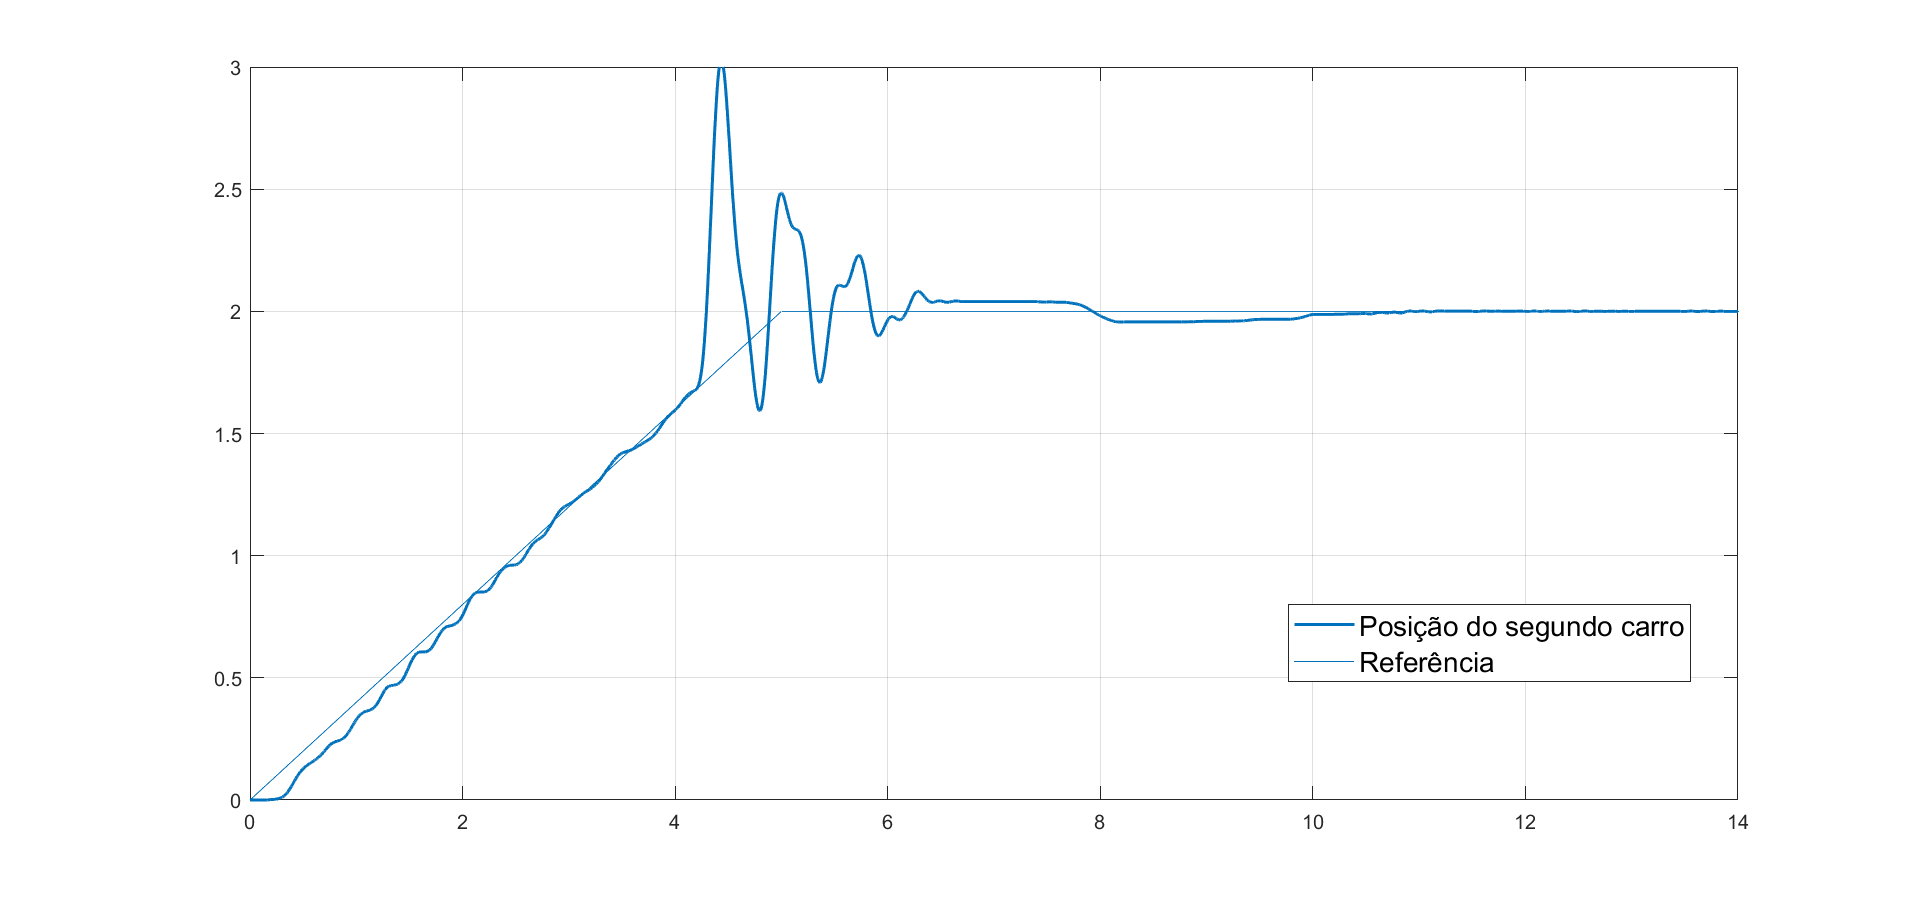
\includegraphics[width=8.4cm]{figures/resultado_teste5.png}    % The printed column width is 8.4 cm.
  \caption{Resposta a rampa com inclinação de 0,5cm/s e saturação em 2cm, carro 1 e 2 com 4 pesos. Fonte: autoral, produzido com \textit{matlab} por meio dos dados coletados na planta.} 
  \label{fig:teste_ramp1_c1_4p_c2_4p}
  \end{center}
\end{figure}

\begin{figure}[!htb]
  \begin{center}
  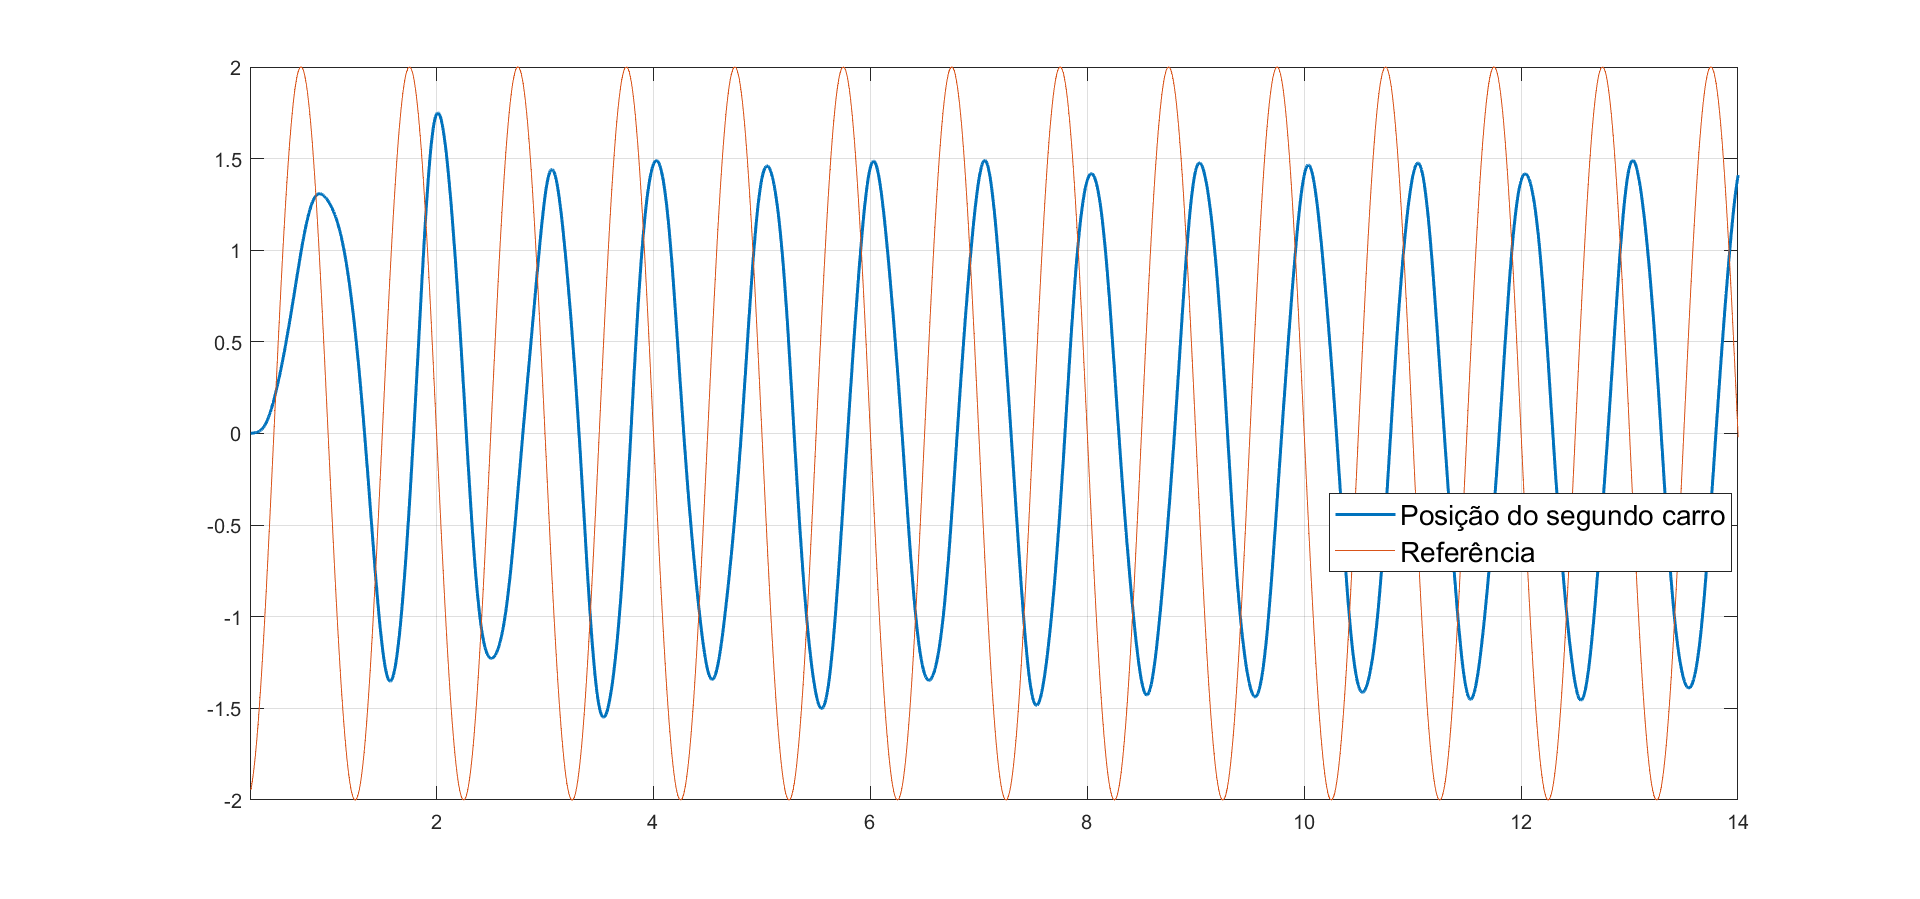
\includegraphics[width=8.4cm]{figures/resultado_teste6.png}    % The printed column width is 8.4 cm.
  \caption{Resposta a senoide com amplitude de 2cm e frequencia de 1 Hz, carro 1 e 2 com 4 pesos. Fonte: autoral, produzido com \textit{matlab} por meio dos dados coletados na planta.} 
  \label{fig:teste_sin1_c1_4p_c2_4p}
  \end{center}
\end{figure}

\section{Conclusão}

Nery vai concluir o trabalho pra gente!

\bibliography{ifacconf}             % bib file to produce the bibliography
                                                     % with bibtex (preferred)
                                                   
%\begin{thebibliography}{xx}  % you can also add the bibliography by hand

%\bibitem[Able(1956)]{Abl:56}
%B.C. Able.
%\newblock Nucleic acid content of microscope.
%\newblock \emph{Nature}, 135:\penalty0 7--9, 1956.

%\bibitem[Able et~al.(1954)Able, Tagg, and Rush]{AbTaRu:54}
%B.C. Able, R.A. Tagg, and M.~Rush.
%\newblock Enzyme-catalyzed cellular transanimations.
%\newblock In A.F. Round, editor, \emph{Advances in Enzymology}, volume~2, pages
%  125--247. Academic Press, New York, 3rd edition, 1954.

%\bibitem[Keohane(1958)]{Keo:58}
%R.~Keohane.
%\newblock \emph{Power and Interdependence: World Politics in Transitions}.
%\newblock Little, Brown \& Co., Boston, 1958.

%\bibitem[Powers(1985)]{Pow:85}
%T.~Powers.
%\newblock Is there a way out?
%\newblock \emph{Harpers}, pages 35--47, June 1985.

%\bibitem[Soukhanov(1992)]{Heritage:92}
%A.~H. Soukhanov, editor.
%\newblock \emph{{The American Heritage. Dictionary of the American Language}}.
%\newblock Houghton Mifflin Company, 1992.

%\end{thebibliography}

\appendix
\section{A summary of Latin grammar}    % Each appendix must have a short title.
\section{Some Latin vocabulary}              % Sections and subsections are supported  
                                                                         % in the appendices.
\end{document}
